% Preamble

% use the beamer document class
\documentclass[hyperref={pdfpagelabels=false}, 14pt]{beamer}
% Text in square brackets is to avoid the warning: Package hyperref Warning: Option `pdfpagelabels’ is turned off (hyperref) because \thepage is undefined. Hyperref stopped early
% See: http://texblog.net/latex-archive/presentations/beamer-warnings/

% to set up the beamer class to use another colour shade, use these lines instead of the one above
%\documentclass[xcolor=dvipsnames]{beamer} 
%\usecolortheme[named=Brown]{structure}

% use Latin Modern fonts
% This also avoids the warnings: LaTeX Font Warning: Font shape `OT1/cmss/m/n’ in size <4> not available (Font) size <5> substituted on input line 6. and: LaTeX Font Warning: Size substitutions with differences  (Font) up to 1.0pt have occurred.
\usepackage{lmodern}

%\usepackage[T1]{fontenc}
%\usepackage[T1]{tipa}
%\usepackage[tipa]{ucs}
\usepackage[utf8x]{inputenc}  % required to allow accented characters like â to appear properly

% use Times New Roman as the default font
%\renewcommand{\rmdefault}{ptm}

% replace the theme lines below with the following line to get rid of most of the colours for handouts
%\usetheme{default}

%\usetheme{Warsaw}
% comment out this line to get a white background and black text on the slide body
%\usecolortheme{albatross}

%\beamertemplateshadingbackground{blue!70}{blue!100}  % gradient full-blue to partial-blue

%\setbeamercolor{structure}{fg=blue!30}
%\setbeamercolor{normal text}{fg=blue!30}
\setbeamertemplate{background canvas}{
\includegraphics [width=\paperwidth,height=\paperheight]{mainpage.jpg}}
%\setbeamertemplate{footline}{\insertframenumber/ \inserttotalframenumber}
\setbeamertemplate{navigation symbols}{}  % hide navigation buttons 

% specify the details to appear on the title page
\title[Autoglossing bilingual data]{\newline\newline Autoglossing bilingual data}
\author{Kevin Donnelly}
\institute{ESRC Centre for Research on Bilingualism, Bangor}
\date{November 2010}

\begin{document}

% build title page
{ % brace to limit the scope of \setbeamertemplate 
\setbeamertemplate{navigation symbols}{}  % hide navigation buttons 
\setbeamertemplate{background canvas}{
\includegraphics [width=\paperwidth,height=\paperheight]{titlepage.jpg}}
\maketitle
} % closing brace

%============================

\section{Introduction}

\subsection{Preamble}

\begin{frame}
\frametitle{\begin{small}\insertframenumber/\inserttotalframenumber\end{small} Acknowledgements}
\begin{itemize}
\item Margaret Deuchar
\item ESRC Centre
\item Brian MacWhinney and Leonid Spektor
\item Colleagues at the ESRC Centre
\end{itemize}
\end{frame}

\subsection{Background}

\begin{frame}
\frametitle{\begin{small}\insertframenumber/\inserttotalframenumber\end{small} Why gloss?}
\begin{itemize}
\item Lexemes and part-of-speech (POS) tags
\item Helps non-native speakers parse the conversation
\item Allows morphological analysis
% Useful to provide if it can be provided
\end{itemize}
\end{frame}

\begin{frame}
\frametitle{\begin{small}\insertframenumber/\inserttotalframenumber\end{small} Example}
\setbeamercolor{uppercol}{fg=white,bg=blue!50}%
\setbeamercolor{lowercol}{fg=black,bg=blue!20}%
\begin{beamerboxesrounded}[upper=uppercol,lower=lowercol,shadow=false]{\textbf{*ALN:} +" oedd@1 o@1 (y)n@1 edrych@1 fath@1 â@1 cael@1 snog@2 pan@1 wnes@1 i@1 basio@1 !}
\begin{small}
\textbf{\%gls:} be.3S.IMP PRON.3SM PRT look.NONFIN kind with have.NONFIN snog when do.1S.PAST PRON.1S pass.NONFIN\\
\textbf{\%eng:} it looked like having a snog when I passed!
\end{small}                                                          
\end{beamerboxesrounded}
\begin{small}
\hfill\textit{(Siarad corpus, stammers4)}
\end{small}
\end{frame}

\begin{frame}
\frametitle{\begin{small}\insertframenumber/\inserttotalframenumber\end{small} Difficulties}
\begin{itemize}
\item Time-consuming
\item Inconsistency and errors
\item Tag choice difficult to revise later
\item No automatic method for small languages
% MOR only available for 11 languages - Cantonese (52m), Danish (5m), Dutch (22m), English (328m), French (68m), German (90m), Hebrew (5m), Japanese(122m), Italian (62m), Mandarin (840m), Spanish (329m)
% POST only available for 4 of these: English, Chinese, Japanese, Spanish
\end{itemize}
\end{frame}

\begin{frame}
\frametitle{\begin{small}\insertframenumber/\inserttotalframenumber\end{small} Questions}
\begin{itemize}
\item If glossing is \textbf{A Good Thing} \dots
\item Can we automate the process?  
\item Can we add value to the texts?
\end{itemize}
\end{frame}

\section{Simplification}

\begin{frame}
\frametitle{}
\begin{center}
\begin{huge}Can we automate the\\\vspace {10 mm} process of glossing?\end{huge}
\end{center}
\end{frame}

\subsection{Overview}

\begin{frame}
\frametitle{\begin{small}\insertframenumber/\inserttotalframenumber\end{small} A sequence \dots}
\begin{itemize}
\item The speech tier = a horizontal stream
  \begin{figure}[h]
  \centering
  
\includegraphics[scale=0.4]{stream.png}
  \end{figure}
\item Additional tiers add vertical depth
  \begin{figure}[h]
  \centering
  
\includegraphics[scale=0.4]{gloss.png}
  \end{figure}
\end{itemize}
\end{frame}

\begin{frame}
\frametitle{\begin{small}\insertframenumber/\inserttotalframenumber\end{small} \dots segmented }
\begin{itemize}
\item Limiting the domain to the word \dots
  \begin{figure}[h]
  \centering
  
\includegraphics[scale=0.4]{boxes1.png}
  \end{figure}
\item \dots provides the basis for glossing automatically
  \begin{figure}[h]
  \centering
  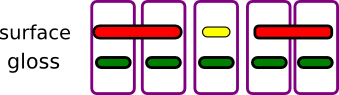
\includegraphics[scale=0.4]{boxes2.png}
  \end{figure}
\end{itemize}
\end{frame}

\subsection{A sample import}

\begin{frame}
\frametitle{\begin{small}\insertframenumber/\inserttotalframenumber\end{small} Process}
\begin{itemize}
\item Read the lines of the chat file into a database table
\item Segment each line into words
\item Look up the words in a digital dictionary
\item Disambiguate using constraint grammar
\item Write the results into a gloss tier, using Leipzig schema 
\end{itemize}
\end{frame}

\begin{frame}
\frametitle{\begin{small}\insertframenumber/\inserttotalframenumber\end{small} Results for Welsh -- manual}
\setbeamercolor{uppercol}{fg=white,bg=blue!50}%
\setbeamercolor{lowercol}{fg=black,bg=blue!20}%
\begin{beamerboxesrounded}[upper=uppercol,lower=lowercol,shadow=false]{\textbf{*ALN:} +" oedd@1 o@1 (y)n@1 edrych@1 fath@1 â@1 cael@1 snog@2 pan@1 wnes@1 i@1 basio@1 !}
\begin{small}
\textbf{\%gls:} be.3S.IMP PRON.3SM PRT look.NONFIN kind with have.NONFIN snog when do.1S.PAST PRON.1S pass.NONFIN\\
\textbf{\%aut:} be.V.3S.IMPERF he.R.M.3S.SPOKEN stative.S look.V.INFIN type.N.M.S.+SM as.C have.V.INFIN snog.V\ .INFIN when.C do.V.1S.PAST.SPOKEN.+SM I.R.1S pass.V\ .INFIN.+SM\\
\textbf{\%eng:} it looked like having a snog when I passed!
% broadly similar, but: mutations are marked; more granular tagging; English tagged as well (snog - though this should probably be a noun here)
\end{small}                                                          
\end{beamerboxesrounded}
\begin{small}
\hfill\textit{(Siarad corpus, stammers4)}
\end{small}
\end{frame}

\begin{frame}
\frametitle{\begin{small}\insertframenumber/\inserttotalframenumber\end{small} Results for Welsh}
\setbeamercolor{uppercol}{fg=white,bg=blue!50}%
\setbeamercolor{lowercol}{fg=black,bg=blue!20}%
\begin{beamerboxesrounded}[upper=uppercol,lower=lowercol,shadow=false]{\textbf{*AVR:} neu dylai bod fi wedi mynd (be)cause@s:en mae (y)n hwyr rŵan .}
\begin{small}
\textbf{\%aut:} or.CY.C ought.CY.V.3S.IMPERF be.CY.V.INFIN I.CY.R.1S after.CY.P go.CY.V.INFIN because.EN.C be.CY.V.3S.PRES stative.CY.S late.CY.A now.CY.B\\
\textbf{\%eng:} or I ought to have gone because it's late now
% use of an explicit language tag
\end{small}                                                          
\end{beamerboxesrounded}
\begin{small}
\hfill\textit{(Patagonia corpus, patagonia2)}
\end{small}
\end{frame}

\begin{frame}
\frametitle{\begin{small}\insertframenumber/\inserttotalframenumber\end{small} Results for Spanish -- MOR}
\setbeamercolor{uppercol}{fg=white,bg=blue!50}%
\setbeamercolor{lowercol}{fg=black,bg=blue!20}%
\begin{beamerboxesrounded}[upper=uppercol,lower=lowercol,shadow=false]{\textbf{*LAR:} +" porque tú me apoyas en todo sabes .}
\begin{small}
\textbf{\%mor:} conj\textbar porque=because pro:per\textbar tú=you pro:per\textbar me=me vpres\textbar apoya-2S\&PRES=support prep\textbar en=in det:indef\textbar todo-MASC=all co\textbar sabes=you\_know\^{}vpres\textbar sabe-2S\&PRES=know .\\
\textbf{\%aut:} because.CONJ you.PRN.SUBJ.MF.2S me.PRN.OBJ\ .MF.1S support.V.2S.PRES on.PREP everything.PRN.M.SG know.V.2S.PRES\\
\textbf{\%eng:} because you support me in everything, you know
\end{small}                                                          
\end{beamerboxesrounded}
\begin{small}
\hfill\textit{(Miami corpus, zeledon14)}
\end{small}
\end{frame}


\begin{frame}
\frametitle{\begin{small}\insertframenumber/\inserttotalframenumber\end{small} Results for Spanish}
\setbeamercolor{uppercol}{fg=white,bg=blue!50}%
\setbeamercolor{lowercol}{fg=black,bg=blue!20}%
\begin{beamerboxesrounded}[upper=uppercol,lower=lowercol,shadow=false]{\textbf{*SEB:} ellos@3 mataban@3 a@3 la@3 gente@3 como@3 nosotros@3 .}
\begin{small}
\textbf{\%aut:} they.PRN.SUBJ.M.3P kill.V.3P.IMPERF~to.PREP the.DET.DEF.F.SG people.N.F.SG like.PREP we.PRN.SUBJ\ .M.1P\\
\textbf{\%eng:} they would kill people like us
\end{small}                                                          
\end{beamerboxesrounded}
\begin{small}
\hfill\textit{(Miami corpus, herring7)}
\end{small}
\end{frame}

\subsection{Assessment}

\begin{frame}
\frametitle{\begin{small}\insertframenumber/\inserttotalframenumber\end{small} Benefits}
\begin{itemize}
\item Speed: 2 minutes/30-minute conversation
\item Consistency: \textit{ychydig} -- ``a bit''/``a little''
% even when they are wrong, they will be consistently wrong
\item Handles any number of languages in one pass
% MOR needs two passes to handle two languages
\item Extensible
% scripting languages are easier than programming languages
% may be simpler for lesser-resourced languages
% dictionary is in a spreadsheet, and the rules use constraint grammar, which is relatively easy to get to grips with
\item Re-uses existing resources and tools
\item Transferable skills
% technology transfer - use tools you can use in other places
\end{itemize}
\end{frame}

\begin{frame}
\frametitle{\begin{small}\insertframenumber/\inserttotalframenumber\end{small} Results}
\begin{center}
\begin{tabular}{ccc}
& \textsc{Welsh} & \textsc{Spanish}\\ \cline{1-3}\noalign{\smallskip}
\textbf{Coverage} (all words) & 88\% & 96\%\\
Tokens & 5224 & 4827\\
\hline\noalign{\smallskip}
\textbf{Correlation} (nouns) & 82\% & 85\%\\
\hline\noalign{\smallskip}
\textbf{Accuracy} (nouns) & 93\% & 97\%\\
Nouns & 459 & 380\\
\hline\noalign{\smallskip}
\begin{small}\textit{Files}\end{small} & \begin{small}\textit{stammers4}\end{small} & \begin{small}\textit{zeledon14}            \end{small}
\end{tabular}
% Welsh: herring7 (12% typo rate), 459 nouns, 5224 tokens; Spanish: splloc, 81 nouns, 470 tokens; zeledon14 (5% typo rate), 380 nouns, 4827 tokens
% MOR does get some things wrong
% Welsh dictionary: 209k items (nouns: 6k); Spanish dictionary: 130k items (nouns: 19k)
\end{center}
\end{frame}

\begin{frame}
\frametitle{\begin{small}\insertframenumber/\inserttotalframenumber\end{small} Drawbacks}
\begin{itemize}
\item Like MOR, still needs checking!
\item Dictionary cleaning can take some time
\item Rules take time to write and test
\end{itemize}
\end{frame}

\section{Adding value}

\begin{frame}
\frametitle{}
\begin{center}
\begin{huge}Can we add value\\\vspace {10 mm} to the texts?\end{huge}
\end{center}
\end{frame}

\subsection{Texts}

\begin{frame}
\frametitle{\begin{small}\insertframenumber/\inserttotalframenumber\end{small} Texts}
\begin{itemize}
\item Check on typos -- proof-reading
% several % typo rate - these lead to misalignment in the autoglosser, but they also cause problems for MOR
\item Consistent glosses
% meddwl not ``consider'' in one place, and ``think'' in another
\item More granular analysis
\item Global tag changes or enrichment
\end{itemize}
\end{frame}

\subsection{Accessibility}

\begin{frame}
\frametitle{\begin{small}\insertframenumber/\inserttotalframenumber\end{small} Accessibility}
  \begin{figure}[h]
  \centering
  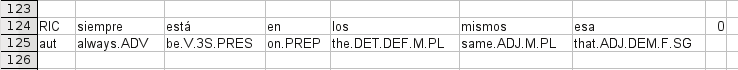
\includegraphics[scale=0.6]{cells.png}
  \end{figure}
\end{frame}

\begin{frame}
\frametitle{\begin{small}\insertframenumber/\inserttotalframenumber\end{small} Accessibility}
\begin{itemize}
\item Interactive webpages (\textit{siarad.org.uk})
% easier mining of the data, no need to install CLAN
  \begin{figure}[h]
  \centering
  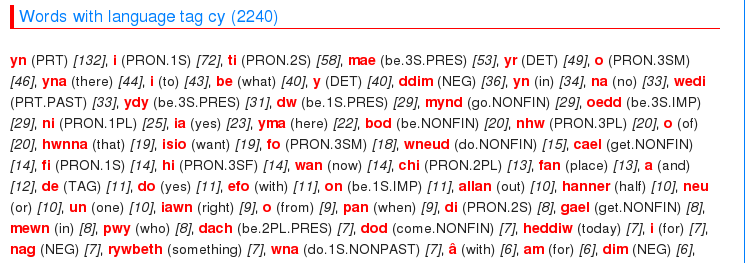
\includegraphics[scale=0.5]{frequency.png}
  \end{figure}
% click on gael, and you get ...
\end{itemize}
\end{frame}

\begin{frame}
\frametitle{\begin{small}\insertframenumber/\inserttotalframenumber\end{small} Accessibility}
  \begin{figure}[h]
  \centering
  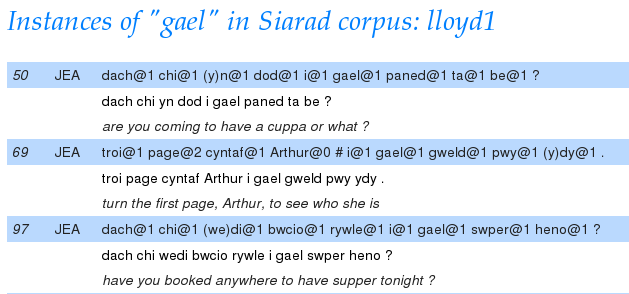
\includegraphics[scale=0.5]{context.png}
  \end{figure}
\begin{itemize}
\item Interface to CLAN queries
% already a very good web interface, but you could aim this more at beginners, with potted queries
\end{itemize}
\end{frame}

\subsection{Data-mining}

\begin{frame}
\frametitle{\begin{small}\insertframenumber/\inserttotalframenumber\end{small} Data-mining}
\begin{itemize}
\item Utterance profiling
  \begin{columns}
  \begin{column}{0.7\textwidth}
    \begin{figure}[h]
    \centering
    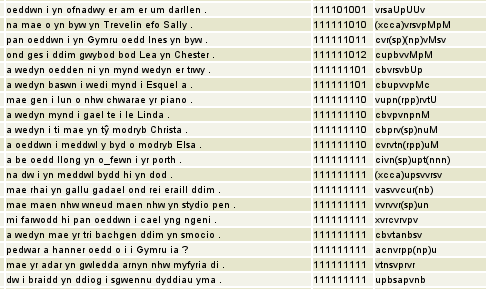
\includegraphics[scale=0.5]{fingerprint.png}
    \end{figure}
  \end{column}
  \begin{column}{0.3\textwidth}
    \begin{figure}[h]
    \centering
    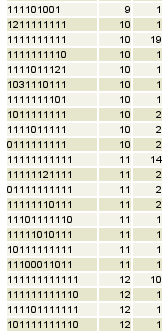
\includegraphics[scale=0.5]{profile.png}
    \end{figure}
  \end{column}
  \end{columns}
\end{itemize}
\end{frame}

\begin{frame}
\frametitle{\begin{small}\insertframenumber/\inserttotalframenumber\end{small} Data-mining}
\begin{itemize}
\item Easier or more detailed statistical analysis
\item N-gram generation (2- or 3-word collocations)
\item Input to statistical machine translation
\end{itemize}
\end{frame}

\begin{frame}
\frametitle{\begin{small}\insertframenumber/\inserttotalframenumber\end{small} Questions}
\begin{itemize}
\item If glossing is \textbf{A Good Thing} \dots
\item Can we automate the process?  
\item Can we add value to the texts?
\end{itemize}
\end{frame}

\end{document}